\chapter{Vulkan Concepts}

\section{Queues, Queue Families And Command Buffers}

\subsection{Command Buffer}

In older graphics APIs, like OpenGL, we simply need to call a function
from our code to execute some operations on the GPU.
This function call causes our application to send a request to the GPU driver.
The GPU driver will then execute the operations we want.
The problem is that it's inefficient to send each request separately.
Vulkan requires us to batch our requests together into a buffer.
This batch is called a command buffer.

\subsection{Queues and Queue Families}

A command buffer is executed by a GPU queue.
A command buffer can contain different kinds of operations, such as graphics
commands, compute commands, transfer commands and so on.
Specific types of commands can only be executed by specific types of queues.
These queue types are called queue families.

There is no connection between a command buffer and a queue or queue family.
There is, although, a connection between the command pool form which a command
buffer is allocated and a queue family.
Each command buffer that takes memory from a given pool can only be submitted
to a queue from the queue family used to create the command pool itself.

\subsection{Command Buffer Execution}

If we want our GPU to execute any kind of commands we need to record a command
buffer and submit it to a proper queue.
When a command buffer is submitted to a queue, all the recorded commands start
being processed by the GPU.
The Vulkan specification guarantees that each command will start execution
in order, but complete their execution out of order.
This is caused by the fact that commands are executed concurrently.
This means that unless we add synchronization ourselves, all commands
in a queue execute out of order.
Commands my get reordered across command buffers and even across different
command buffer submissions.
The GPU only sees a linear stream of commands.
It's a common pitfall to assume that splitting command buffers or submits adds
some sort of automatic synchronization for us.

\section{Image Layouts And Layout Transitions}

Images are used for different purposes.
They can be used as render targets, as textures or even for data transfers.
When we create an image we also specify its usage flags.
These flags indicate the different types of operations we want to perform
on the image.
Image usage is not the only thing we need to specify.
Each type of operation is linked to a specific image layout.
We could also use a general layout that supports all operations, but this
would be inefficient.
We usually change the image's layout before we perform a given type of
operation.
We explicitly transition an image's layout using an image memory barrier.
We implicitly transition an image's layout using render pass' subpasses.

\section{Swapchain}

A swapchain is nothing but a set of images that can be presented on the screen.
Presenting an image means displaying it.
In practice, we present an image by giving it back to the OS's presentation engine.
We use a present mode to configure how images are internally processed by
the presentation engine, and how they are displayed to the screen.

\subsection{Immediate}

This is the simplest present mode.
Using this present mode, the presentation engine reserves only one swapchain
image at a time.
This image is the one that is currently displayed on the screen.
When we execute a present request, the presentation engine releases
the current displayed image and acquires the one we want to present.
The problem with this present mode is that the presentation engine doesn't
wait for our monitor to finish reading the image.
This can cause a graphical artifact known as tearing.

\subsection{FIFO}

Using this present mode, the presentation engine reserves at least two
swapchain images at a time.
One swapchain image is the one that is currently being displayed.
One or more swapchain images that we can render into.
When we execute a present request, the presentation engine acquires
the image we want to present and puts it into a queue.
When the monitor finishes displaying the current image, the presentation engine
removes it from the head of the queue, releasing it, and then starts
presenting the next image in the queue.
Doing this we avoid tearing, but another problem arises.
When the queue is full, our application doesn't have other images that can
render into, hence it has to wait for the presentation engine to release the
currently presented image.

\subsection{Mailbox}

Using this present mode, the presentation engine reserves at least three
swapchain images.
One image that is being presented, one image that waits for the current image
to be presented and one or more images that can be rendered into.
When we issue a present request, the presentation engine replaces the
image that is waiting to be presented, releasing it, with the one we want
to present.
This technique solves tearing, and also doesn't require our application to
block execution, since there is always an image we can render into.

\section{Render Pass And Framebuffer}

\subsection{Render Pass}

A render pass describes a set of images, also called attachments, required
for drawing operations.
A render pass also describes a series of subpasses that drawing operations
are ordered into.

A subpass collects drawing operations that use the same attachments.
Each of these drawing operations may use some attachments as inputs,
reding data from them, and other attachments as outputs, writing data into them.

\subsection{Framebuffer}

A framebuffer is the set of images a render pass instance operates on.
Hence, a framebuffer collects the actual attachments used by a render pass.

\section{Pipeline State Object}

The graphics pipeline is composed by a series of stages.
Each performing a given operation.
Some stages are programmable by us, while other stages can only be
partially configured.
OpenGL allows us to change the stages' configuration whenever we want.
In Vulkan we can't do this.
We must bundle our pipeline configuration into one monolithic object
that represent the pipeline's state in its entirety.
This comes from performance considerations.
Changing the configuration of just one single stage may require a lot of
operations in the background at runtime.
This may cause noticeable slowdowns in our application.
In Vulkan we avoid this by creating ahead of time multiple pipeline state
objects, each representing a given set of stages' configurations.

\section{Descriptors And Descriptor Sets}

Resources used inside shaders are called descriptors.
Vulkan doesn't allow us to directly provide descriptors to shaders.
We must aggregate descriptors in an object called descriptor set.
We can place whatever resources we want inside a descriptor set,
but we have to respect the structure of the set.
The structure of a descriptor set describes what types of resources
can be contained inside the set, the number of each of these resources and
their order.
This description is provided by a descriptor set layout.
In summary, descriptor sets are objects in which we store resources' handles,
while descriptor set layouts define how to interpret the data inside a
descriptor set.

\begin{figure}[H]
    \centering
    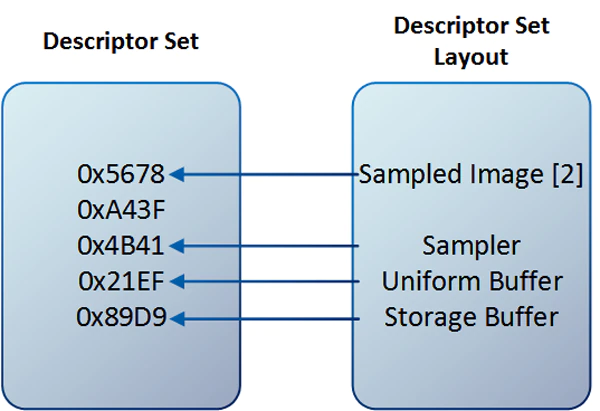
\includegraphics[scale=0.30]{images/ApVulkanConcepts/DescriptorSetAndSetLayout.png}
    \caption{Descriptor set and descriptor set layout}
    \label{fig::DescriptorSetAndSetLaytout}
\end{figure}
